%
% File acl2017.tex
%
%% Based on the style files for ACL-2015, with some improvements
%%  taken from the NAACL-2016 style
%% Based on the style files for ACL-2014, which were, in turn,
%% based on ACL-2013, ACL-2012, ACL-2011, ACL-2010, ACL-IJCNLP-2009,
%% EACL-2009, IJCNLP-2008...
%% Based on the style files for EACL 2006 by 
%%e.agirre@ehu.es or Sergi.Balari@uab.es
%% and that of ACL 08 by Joakim Nivre and Noah Smith

\documentclass[11pt,a4paper]{article}
\usepackage[hyperref]{acl2017}
\usepackage{times}
\usepackage{latexsym}
\usepackage{xcolor}
\usepackage[normalem]{ulem}
\usepackage{url}
\usepackage{pgfplots}
\usepackage{tikz}

\definecolor{forestgreen}{rgb}{0.13, 0.55, 0.13}

% Define bar chart colors
%
\definecolor{bblue}{HTML}{4F81BD}
\definecolor{rred}{HTML}{C0504D}
\definecolor{ggreen}{HTML}{9BBB59}
\definecolor{ppurple}{HTML}{9F4C7C}

%\aclfinalcopy % Uncomment this line for the final submission
%\def\aclpaperid{***} %  Enter the acl Paper ID here

%\setlength\titlebox{5cm}
% You can expand the titlebox if you need extra space
% to show all the authors. Please do not make the titlebox
% smaller than 5cm (the original size); we will check this
% in the camera-ready version and ask you to change it back.

\newcommand\BibTeX{B{\sc ib}\TeX}

% Writing macros
\newcommand{\secref}[1]{Section~\ref{ssec:#1}}
\newcommand{\figref}[1]{Figure~\ref{#1}}
\newcommand{\tabref}[1]{Table~\ref{#1}}
\newcommand{\isection}[2]{\section{#1}\label{ssec:#2}}
\newcommand{\isectionb}[1]{\section{#1}\label{ssec:#1}}
\newcommand{\com}[1]{}

% Editing macros
\newcommand{\ms}[1]{{\color{cyan}\{\textit{#1}\}$_{ms}$}}
\newcommand{\roy}[1]{\footnote{\color{red}{\textbf{Roy: #1}}}}
\newcommand{\royb}[2]{{\color{red}{\sout{#1}}}{\color{green}{#2}}}
\newcommand{\royc}[3]{\royb{#1}{#2}\roy{#3}}

%\renewcommand{\ms}[1]{}
%\renewcommand{\roy}[1]{}
%\renewcommand{\royb}[1]{}
%\renewcommand{\royc}[1]{}


\title{???}

\author{First Author \\
  Affiliation / Address line 1 \\
  Affiliation / Address line 2 \\
  Affiliation / Address line 3 \\
  {\tt email@domain} \\\And
  Second Author \\
  Affiliation / Address line 1 \\
  Affiliation / Address line 2 \\
  Affiliation / Address line 3 \\
  {\tt email@domain} \\}

\date{}

\begin{document}
\maketitle
\begin{abstract}
People's writing style is affected by many factors, including topics, sentiment, and individual personality. 
In this paper we show that writing tasks that impose constraints on the writer result in the author adopting a  different writing style compared to tasks that do not.
As a case study, we experiment with a recently published machine reading task: the story cloze task \cite{Mostafazadeh:2016}. 
In this task, annotators were asked to generate two sentences: one which makes sense given a previous paragraph and another which doesn't.
We show that a linear classifier, which applies only simple style features, such as sentence length and character n-grams, obtains state-of-the-art results on the task,
substantially higher than sophisticated deep learning models.
Importantly, our model doesn't even look at the previous paragraph, just the two candidate sentences, which, out of context, differ only in the constraint put on the authors. 
Our results indicate that such constraints dramatically affect the way people write. 
They also suggest that careful attention to the instructions given to the authors needs to taken when designing new NLP tasks.

\end{abstract}

\section{Introduction}
Writing style is defined as the the author's choice of words, spelling, grammar and punctuation.\footnote{\url{https://en.wikipedia.org/wiki/Writing_style}}
It is often affected by inter-writer factors such as age \cite{Schler:2006}, gender \cite{Argamon:2003}, native language \cite{Koppel:2005}, or mere personality \cite{Stamatatos:2009}, but also by other parameters such as the sentiment of the text \cite{Davidov:2010} and its level of sarcasm \cite{Tsur:2010}.  
In this paper we study to what extent is writing style affected by more intricate factors, such as the type of constraints put on the author. 

As a testbed, we experiment with the story cloze task \cite{Mostafazadeh:2016}. 
In this task, authors were asked to write five-sentence self-contained stories.
Following, the stories were given to another group of authors, who were shown only the first four sentences of each story, 
and were asked to write two one-sentence endings for it: a {\it correct} ending, and a {\it wrong} ending.
The goal of the task is to determine which of the endings is the correct one.
\tabref{ROC-example} shows an example of an original story, a {\it correct} story and a {\it wrong} story.

\begin{table}[!t]
%\small
\begin{tabular}{|p{1.3cm}|p{5.6cm}|} \hline
{\bf Type} & {\bf Example} \\ \hline
{\it Original} story & My mother loves clocks that chime.	Her house is full of them.	She sets them each a little different so she can hear them chime.	It sounds like a bell tower during a wedding in her house all day.	{\color{blue}{When I visit I stop them or I'd never be able to sleep at night.}} \\ \hline
{\it Correct} story & Kathy went shopping.	She found a pair of great shoes.	The shoes were \$300.	She bought the shoes.	{\color{forestgreen}{She felt buyer's remorse after the purchase.}} \\ \hline
{\it Wrong} story & Kathy went shopping.	She found a pair of great shoes.	The shoes were \$300.	She bought the shoes.	{\color{red}{Kathy hated buying shoes.}} \\ \hline
\end{tabular}
\caption{\label{ROC-example}}
Examples of stories from the story cloze task. The first row shows an original story written by one author. 
The second and third row show two endings of the same story: a {\it correct} ending and a {\it wrong} one.
%\end{center}
\end{table}


Interestingly, although originally intended to be a machine reading task, the compilation of this task raises several research questions which seem to differ from the original intent of the designers.
First, do authors use different style when asked to write a {\it correct} sentence, compared to a {\it wrong} sentence?
Second, do authors use different style when writing the ending as part of their own five sentence story, compared to reading four sentences, and then writing a standalone ({\it correct}) ending?

Our experiments indicate that the answer to both questions is positive. 
We train a linear classifier, using simple stylistic features, such as sentence length, character n-grams and PoS counts. 
First, we show that on a balanced dataset (random guess is 50\%) our classifier distinguishes between {\it correct} and {\it wrong} sentences in 64.5\% of the cases. 
Importantly, the classifier is trained {\bf only} on the last sentences, and does not consider the four input sentences.
%It is also trained on a set of positive samples and a set of negative ones, rather than pairs of (positive, negative) pairs, as in the original story cloze task.
Second, when trained to distinguish between original endings and new ({\it correct}) endings, the classifier obtains 70.9\% accuracy. 


In order to estimate the quality of our results, we turn back to the story cloze task.
Using our classifier, we are able to obtain 71.5\% accuracy on the task, a 11.6\% improvement compared to the published state-of-the-art results \cite{Salle:2016}.\footnote{Recently, a shared task for the story cloze task has been published (\url{https://competitions.codalab.org/competitions/15333}). 
At the time of submission, the leading results is 71.1\%, which is much closer to our results, although still inferior.
No details about the methods used to generate this result are available.}
An ablation study shows that the style differences are realized in syntactic features (such as the over/under use of coordination words like ``and'' and ``but''),
but that sentiment also plays an important role in the writing style differences.
For instance, one of the key features for distinguishing between correct and wrong sentences is the over-representation of the word ``hate" in the latter.

\com{Our results suggest that writing style is affected by the the writer's state of mind.
Writing a sentence intended to be {\it wrong} turns out quite differently than a sentence intended to be {\it correct}. 
Similarly, writing a sentence as part of the story is different from reading a story, and then writing the final sentence.}

Our results may have a wide impact on a range of fields. 
First, they have the potential to shed light on cognitive processes that take place in the brain during writing.
Second, our results might have a more practical value in an era when fake news are becoming prominent,
as they suggest that these might have different style compared to real news.
Third, the results presented here also provide valuable lessons for designing new NLP tasks,
both in terms of the potential impact of even the smallest details, and the need to carefully run baseline models.
%Although \cite{Mostafazadeh:2016} seem to have put a lot of effort into designing the task, 
%addressing many potential methodological flaws (see \secref{ROC_Story}), the importance of a few allegedly minor details were underestimated. 
%We show that these details are actually very significant.

Finally, one interesting question that remains open is whether state-of-the-art machine reading tools, for which this task was designed, 
capture in fact the same stylistic features as our linear classifier. 
We show that this is not the case. 
We train a neural language model on the original five sentence training corpus, and then compute the language probability of each of the candidates answers. 
We add the numbers as features in our linear classifier, and get an additional 3.6\% improvement (75.1\%).

The remainder of this paper is organized as follows. In \secref{ROC_Story} we introduce the cloze story task.
We present our model and our experiments at sections \ref{ssec:Model} and \ref{ssec:Experiments} respectively.
Sections \ref{ssec:Ablation} and \ref{ssec:Discussion} present an ablation study and a discussion, while \secref{Related}  surveys related work. 
We conclude at \secref{Conclusion}.

\isection{The Cloze Story Task}{ROC_Story}
%\roy{High level on first paragraph: much better, but still not enough connection to our story. You need to be explicit as to why we chose this task. Our work is currently not mentioned at all}
To understand how constrained writing affects writing style, we focus on the \textit{Story Cloze Task} \cite{Mostafazadeh:2016}. We exploit various interesting properties of the associated dataset and achieve state-of-the-art performance on the task.

Originally, the task was developed as an effort to facilitate representation and learning of commonsense knowledge. For that purpose, \citet{Mostafazadeh:2016} crowdsourced the collection of two types of datasets: the \textit{ROC Stories} and the \textit{Story Cloze test sets}.


\paragraph{ROC Stories}
consist of $98,163$ % \roy{Minor, but still: writing the number inside dollar signs adds a white space in the pdf. This is a bit annoying, and also potentially confusing, as in the next case you use it below (3,744 something)}
five-sentence commonsense stories, collected on Amazon Mechanical Turk (AMT). Workers were instructed to write a coherent story where something happens, and with%\roy{``and with'' doesn't sound right here. rephrase}
a clear beginning and end. To collect a broad spectrum of commonsense knowledge, there was no imposed subject for the stories.
\paragraph{Story Cloze}%\roy{say something general first before diving into details} 
test sets consist of $3,744$ short stories, each with one ``right'' and one ``wrong'' ending, also collected on AMT.
Presented with the first four sentences of a ROC story, workers were asked to write a ``right'' and a ``wrong'' ending. Both endings had to complete the story using one of the characters in it, and when read out of context, the ending had to be ``realistic and sensible'' \cite{Mostafazadeh:2016}.

The resulting stories, matched with each ending, were then individually rated for coherence and meaningfulness by AMT workers. Only stories rated as simultaneaously coherent with a ``right'' ending and neutral with a ``wrong'' ending were selected for the test. It is worth noting that workers rated the stories as a whole, not the endings; no selection was done on the endings alone.

\paragraph{Design.}
In this task, training (ROC Stories) and test (Story Cloze) data were created differently.
%The task was designed such that the ROC stories would be used as training data and the Story Cloze stories as validation and test sets, i.e. the training and test data were created differently. 
The ROC Stories were written by one author, and only have one ``right'' ending, whereas the Story Cloze stories have two endings, neither or which were written by the author of the rest of the story. Furthermore, \citet{Mostafazadeh:2016} made sure the Story Cloze endings would be hard to distinguish automatically, as each pair of endings was written by the same author. We show that, as a result of these design choices, the style of the ROC stories is rather different from the Story Cloze stories.

\paragraph{Benchmarks.} While the Story Cloze test is now the LSDSem `17 Shared Task and was proposed as a testbed for vector-space evaluation \cite{mostafazadeh2016story}, reported performance isn't far from a random baseline. \citet{Mostafazadeh:2016} implemented various benchmarks trained on the ROC Stories, using surface level features as well as narrative-informed ones. Compared to similar tasks \cite{hermann2015teaching,rajpurkar2016squad,bowman2015large}, the benchmarks perform relatively poorly, indicating that high performance is hard to achieve.
To the best of our knowledge, no training has been done on pairs of endings.




%\roy{Other things to talk about (not necessarily in that order): 
%1. no training corpus for the task. That is, the training set (a) does not contain negative example (just positive), and (b) was not generated in the same way as the positive test samples. Here you need to explicitly say that we show that we show that the training and test sets use very different styles.
%2. Maybe talk about the shared task, as well as their RepEval paper, which suggested this task as a vector-space evaluation measure?
%3. Say that the authors did an extensive work in order to  assure that the positive and negative samples are not easily distinguishable: for each pair, both endings were written by the same author (you addressed this earlier, but this seems like a better location), they tried an extensive set of baselines, showing all don't surpass a random baseline by much. Maybe now you can briefly mention the benchmarks, saying that several baselines were presented in the papers. All benchmarks attempted to learn the connection between the previous paragraph and the ending, and all performed near chance level.. However, no baseline looked at the endings independently. 
%Then you can add the benchmark text below, and conclude that this indicates that this task is well designed and hard and the one hand, but might also point to potential disagreements between the train and the test data, which we highlight in this paper.}


\isectionb{Model}

The goal of this paper is to determine to what extent does constraining authors in their writing assignments lead to them adopting different writing styles. 
In order to answer these questions, we use simple, classic NLP tools, which have been shown to be very effective for recognizing style (see \secref{Related}).
We describe our model below.

We train a linear SVM classifier to distinguish between different endings. 
Each feature vector is computed using the words in one ending, without considering earlier parts of the story. 
We use the following style features.

\begin{itemize}
\item\textit{\textbf{Length~}} The number of words in the sentence.
\item\textit{\textbf{Word n-grams~}} We use sequences of 1-5 words. Following \cite{Tsur:2010,Schwartz:2013}, we distinguish between high frequency and low frequency words. 
Specifically, we replace content words with their part-of-speech tags (Nouns, Verbs, Adjectives and Adverbs).
\item\textit{\textbf{Character n-grams~}} Character n-grams are one of the most useful features in identifying author style \cite{Stamatatos:2009}. 
We used character 5-grams.
\end{itemize}

\isectionb{Experiments}
We design two experiments to answer our research questions. 
The first is an attempt to distinguish between {\it correct} and {\it wrong} endings.
The second attempts to distinguish between original endings and new {\it correct} endings.
We describe both experiments below.

\paragraph{Experiment 1: Correct/Wrong Endings.}
The goal of this experiment is to measure to what extent  style features capture differences between {\it correct} and {\it wrong} endings.
As the cloze story task doesn't have a training corpus for the {\it correct} and {\it wrong} endings, we use the development set as our training set. 
We split it (90/10) into our training and development set. We keep the story cloze test set as is.
The final size of our training/development/test sizes are 3366/374/3742, respectively. 

We take  {\it correct} endings as positive samples and {\it wrong} endings as our negative examples. 
By ignoring the coupling between {\it correct}/{\it wrong} pairs, we are able make a more general claim about the style used when writing each of the tasks.

We add a special START symbol at the beginning of each sentence. 
For computing our features, we keep n-gram (character or word) features that occur at least five times in the training set.\footnote{Virtually all sentences end with a period, so no need for an END token}
For the PoS features, we tag each sentence with the Spacy PoS tagger.\footnote{\url{spacy.io/}}
We use  sklearn's LinearSVC SVM implementation\footnote{\url{scikit-learn.org/stable/modules/generated/sklearn.svm.LinearSVC.html}} 
with L2 loss. We grid search the regularization parameter on our development set. 

\paragraph{Experiment 2: Original/New Endings.}

Here the goal is to measure whether writing the ending as part of a story imposes different style compared to writing a ({\it correct}) ending to an existing story.
We use the endings of the original ROC stories as our {\it original} training samples and {\it correct} endings from the ROC stories development set as {\it new} training samples.
As there are far more {\it original} samples than {\it new} ones, we randomly select $N$ {\it original} samples, where $N$ is the number of {\it new} samples,
such that we have balanced labels in our training, validation and test sets.
We apply the same experimental decisions as in Experiment 1, and repeat this process 5 times while reporting the average.

\paragraph{Results.}
\figref{results} shows our results.
Results show that for Experiment 1, our model obtains results well above a random baseline -- 64.5\% classification accuracy. 
For Experiment 2, we get even higher results -- 70.9\%. 
These numbers indicate that these different writing tasks clearly impose a different writing style on authors. 

As a complementary experiment, we measured whether these style differences are additive. 
That is, whether the style differences between {\it correct} endings and {\it wrong} ones are different from the differences between {\it correct} and {\it original} endings.
We repeated Experiment 2, this time comparing between {\it original} and {\it wrong} sentences. 
Our hypothesis is that differences would be even clearer. 
Our results (\figref{results}) show that this is indeed the case: the classifier's accuracy jumps to 78\%.

\begin{figure}
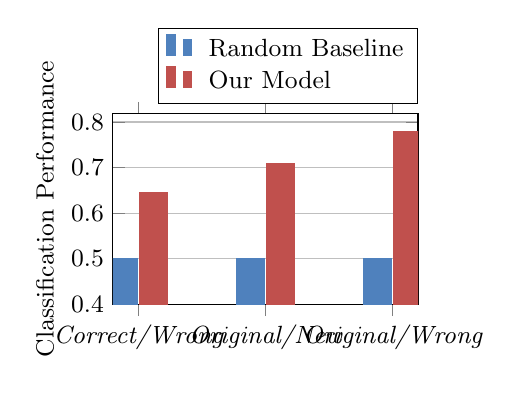
\begin{tikzpicture}
\small
    \begin{axis}[
        width  = 0.45*\textwidth,
        height = 4cm,
      %  major x tick style = transparent,
        ybar=2*\pgflinewidth,
       % bar width=14pt,
        ymajorgrids = true,
        ylabel = {Classification Performance},
        symbolic x coords={{\it Correct/Wrong}, {\it Original/New}, {\it Original/Wrong}},
        xtick = data,
        scaled y ticks = false,
        %enlarge x limits=0.25,
        ymin=0.4,
        legend cell align=left,
        legend style={
                at={(1,1.05)},
                anchor=south east,
                column sep=1ex
        }
    ]
        \addplot[style={bblue,fill=bblue,mark=none}]
            coordinates {({\it Correct/Wrong}, 0.5) ({\it Original/New}, 0.5) ({\it Original/Wrong},.5)};

        \addplot[style={rred,fill=rred,mark=none}]
            coordinates {({\it Correct/Wrong}, 0.645) ({\it Original/New}, 0.709) ({\it Original/Wrong},0.78)};

        \legend{Random Baseline, Our Model}
    \end{axis}
\end{tikzpicture}
\caption{\label{results} Results of  experiments 1 and 2 (left two charts). 
Rightmost experiment shows a control experiment which classifies {\it original} endings vs \textit{\textbf{wrong}} endings. }
\end{figure}


\paragraph{Story Cloze.}
Results of Experiment 1 indicate that {\it correct} and {\it wrong} endings are characterized by different styles.
In order to estimate the quality of our classification results, we tackle the story cloze task using our classifier.
This classification task is much more constrained than Experiment 1, as here the task is given two endings, which one is {\it correct} and which is {\it wrong}.
In order to solve the task, we use the output of our trained classifier. 
For each pair of endings $e_1,e_2$, if both endings have different classification labels, we keep these labels. 
If they share the same label, we use the classifier confidence level as a deciding factor: the label of the one with the lower confidence is reversed. 

\tabref{cloze_results} shows our results on the story cloze test set. Our classifier obtains 71.5\% accuracy, which is 11.6\% better than the published state-of-the-art result on the task.
Importantly, unlike previous approaches, our classifier does not require the story corpus training data, and in fact doesn't even look at the first four sentences of the story in question.
These numbers indicate that the styles between {\it correct} and {\it wrong} are indeed very different.

Other than the published works that tackled this task, a few  recent works published their results in the LSDSem shared task website.\footnote{\url{https://competitions.codalab.org/competitions/15333}} 
As to the time of submission, our results are still state-of-the-art (though by a much smaller margin). No other information other than the name of the group and their results is available.

\begin{table}[!t]
\begin{center}
%\small
\begin{tabular}{|c|c|} \hline
{\bf Model} & {\bf Results} \\ \hline
{DSSM} \cite{Mostafazadeh:2016} & 0.585 \\ \hline
{ LexVec} \cite{Salle:2016} & 0.599 \\ \hline
{RNN}		& 0.681 \\ \hline
{\bf Our Model} & {\bf 0.715} \\ \hline
{\bf Combined (Our model, RNN)} & {\bf 0.751} \\ \hline\hline
{ Niko (shared task)}	& 0.7\\ \hline\hline
{ tbmihaylov (shared task)} & 0.711\\ \hline\hline
Human judgment & 1 \\ \hline
\end{tabular}
\end{center}
\caption{\label{cloze_results}}
Results on the test set of the cloze story task. 
Upper part are published results (Lexvec results are taken from \cite{Speer:2016}).
Bottom part are taken from the cloze task shared task webpage.
\end{table}




\isection{Ablation Study}{Ablation}



\paragraph{Most Discriminative Feature Types.}
A natural question that follows this study is which features are most helpful in making predictions about writing style. 
To answer this question, we re-ran Experiment 1 with different sub-groups of features. 
\tabref{subgroups} shows our results. Results clearly show that  character n-grams are the most effective style predictors, reaching within less than 2\% of the full model.
These findings are in line with previous works that used character n-grams along with other types of features to predict writing  style \cite{Schwartz:2013}.


\begin{table}[!t]
\begin{center}
%\small
\begin{tabular}{|c|c|} \hline
{\bf Feature Type} & {\bf Result}\\ \hline
Word n-grams & 0.646 \\ \hline
Char n-grams & 0.699 \\ \hline
Full Model & 0.715 \\ \hline

\end{tabular}
\end{center}
\caption{\label{subgroups}}
Results on Experiment 1 with different types of features.
\end{table}

\paragraph{Most Salient Features.}
In order to understand which features were most salient, we repeated Experiment 1, this time running SVM with L1 norm, such that it generates a sparse separating hyperplane. 
This came at a minor cost of less than 2\% in performance compared to our L2 results (0.697 compared to 0.715).  
\tabref{features} shows the 5 features with the highest positive and negative weights in the hyperplane. 
These correspond to the 5 most salient features for {\it correct} and {\it wrong} endings, respectively.

The table shows a few interesting trends. 
First, some syntactic features play become salient when authors are asked to write {\it wrong} vs. {\it correct} endings.
For instance, {\it correct} endings are more likely to the coordinator ``but'', while {\it wrong} ones would prefer to use ``and''.

More interestingly, {\it correct} endings are likely to use positive words (e.g., `` bett'', which in all cases stands for `` bett{\bf er}''), while  {\it wrong} endings would use negative words (e.g., `` hate''). 
The idea that  sentiment would play a role in this task was suggested in the original story cloze paper, where two sentiment-based baselines were evaluated. 
However, these baselines measured the relative sentiment between the ending and the previous sentences, and did not test whether there is a general tendency of the {\it wrong} endings to have a negative sentiment, and the {\it correct} one to have a positive sentiment.
Indeed, the performance of both these baselines was roughly chance-level.


\begin{table}[!t]
\begin{center}
%\small
\begin{tabular}{|c|c|} \hline
{\bf Positive} & {\bf Negative}\\ \hline
` time' & `ed of'\\ \hline
` bett' & `and d'\\ \hline
`found' & `threw'\\ \hline
`but' & `ever '\\ \hline
`ally ' & ` hate'\\ \hline

\end{tabular}
\end{center}
\caption{\label{features}}
The top 5 most discriminative features for predicting {\it correct} (Positive)  and {\it wrong} (Negative) endings.\end{table}

\[add\ control\ experiments\]

\paragraph{Neural Language Model.}
%~\ms{This needs to be placed somewhere else LOL}
%~\ms{Below is a messy dump of all the hyper parameters... Didn't know how many details were needed}
%\roy{The level of description seems fine (we might remove some of them if space is an issue, but for now it's good. What I'm missing here are (a) an introductory 1-2  sentences to what are we doing here (I realize that it is not 100\% clear from the intro what is the role of these experiments other than showing that we have STOA results, so this can come later\\
%(b) A one-sentence description of your model. Currently, there is no clear separation between the model (RNN using LSTM) and the technical details. 
%Some general description of the model, and specifically the motivation behind (nothing fancy, just saying that we applied state-of-the-art LM tools, 
%which resemble the tools the authors had in mind when they designed the task).}

We investigate whether our model can benefit from state-of-the-art text comprehension models, for which this task was designed. Specifically, we train a recurrent language model (RLM) \cite{mikolov2010recurrent}. % , which have been shown to help
Unlike the model in this paper, which only considers the story endings, this language model harnesses the ROC Stories training set as intended by the authors, which consists of unsupervised, single-ending stories. Adding in the features from the language model further boosts our performance on the Story Cloze task.

% To leverage the genre of these short stories,\roy{Not sure this is the best introductory sentence, but you can leave it to me if you can't find anything better} we train a recurrent language model (RLM) \cite{mikolov2010recurrent},\roy{don't start with the details, but with the high level. We wanted wether our model can be combined with state-of-the-art text comprehension models, for which this task was designed. {\bf Specifically}, we train an RLM \dots}  which are used to achieve state-of-the-art performance on various tasks (e.g. machine translation)\roy{citation required}. 
%Training this RLM on the ROC stories, we harness the unsupervised, single-ended stories\roy{I would frame it differently. Unlike the model suggested in this paper, which only considers the endings, this model harnesses the training set as intended by the authors, which is composed of unsupervised, single-ended stories}, which boosts performance on the Story Cloze task.\roy{In what sense does it boost performance? we get STOA results without it...}

We trained an RLM using a single-layer LSTM \cite{hochreiter1997long} of hidden dimension $h=512$.
We used the ROC Stories for training, setting aside $10\%$ for validation of the language model. We replaced all words occurring less than 3 times by a special out-of-vocabulary character, yielding a vocabulary size of $|V|=21,582$.
Only during training, we applied a dropout rate of 60\% while running the LSTM over all 5 sentences of the stories. Using AdamOptimizer \cite{kingma2014adam} and a learning rate of $\eta=.001$, we trained with backpropagation on cross-entropy. % minibatches of $50$ stories.
% h=512, dropout rate of 60%, V=21582, 10% validation set


% Eval
On its own, our neural language model performs moderately on the Story Cloze test. As hinted at by the creators of this task, simple language models aren't enough to do well. In fact, using our neural LM and selecting endings based on $p_\theta(ending|story)$, we obtain only $55.0\%$ accuracy. When using the likelihood ratio $\frac{p_\theta(ending|story)}{p_\theta(ending)}$ to select endings, we obtain $68.1\%$ (see \tabref{cloze_results}).

We notice that these features boosts perfromance by $3.6\%$, indicating that harnessing the unsupervised data from the ROC Stories complements using stylistic differences in the two endings in the Story Cloze stories.
% \roy{Now you need to discuss our results and what they mean. You can point to \tabref{cloze_results}}

% \roy{no, this is not why we include these as features (at least not in this paper:). It's because we want to see whether the different approaches are complementary.}


% To construct features for the Story Cloze task, we scored each of the two endings using our neural language model. We computed the probability of each ending given the first four sentences $p_\theta(ending|story)$, as well as the probability of the endings out of context $p_\theta(ending)$. We also included the likelihood ratio $\frac{p_\theta(ending|story)}{p_\theta(ending)}$ into our classifier.
%\roy{This will probably change once we have the rest of the paper, but generally a few things that are missing:(a) performance of the model as a standalone (both how we evaluated it and how much it got). (b) modifying this paragraph to indicate that in order to combine between the style features presented in this paper and this model, we did the above.(c) results of the combination (75.1\%).\\These numbers might best fit in a small table.}

\isectionb{Discussion}



\isection{Related Work}{Related}

\begin{itemize}
\item Different style application (as in introduction). Also include deception works (Yejin has 1-2 papers on it). 
\item Machine reading papers? 
\item \ms{Pennebaker's work on function words? they link function words to psychological aspects}
\end{itemize}


\isectionb{Conclusion}




% include your own bib file like this:
%\bibliographystyle{acl}
%\bibliography{acl2017}

\newpage
\bibliography{acl2017}
\bibliographystyle{acl_natbib}

\end{document}
